\documentclass[11pt,oneside,a4paper]{article}
\usepackage{graphicx}
\usepackage{float}
\usepackage{booktabs}
\usepackage{array}
\usepackage{caption}
\usepackage{subcaption}
\usepackage{amsmath}
\usepackage{amsfonts}
\usepackage{amssymb}
\usepackage[usenames]{color}
\usepackage{xcolor}
\usepackage{bbm}
\usepackage[bookmarks,pdfstartview=FitH,a4paper,pdfborder={0 0 0}]{hyperref}
\usepackage{textcomp}
\usepackage{course}
\usepackage{fancyhdr}
\pagestyle{fancy}
\usepackage[acronym]{glossaries}

\graphicspath{{figures/}}

\newacronym{pppn}{PPPN}{Partially Principal Protected Note}
\newacronym{jpm}{JPM}{JPMorgan Chase \& Co}

\renewcommand{\sectionmark}[1]{\markboth{#1}{#1}}
\renewcommand{\subsectionmark}[1]{\markright{#1}}

\fancyhf{}
\fancyhead[RO]{\nouppercase{\footnotesize\sc\leftmark\ \hrulefill\ \thepage}}
\fancyhead[RE]{\nouppercase{\footnotesize\sc\thepage\ \hrulefill\ }}
\renewcommand{\headrulewidth}{0pt}

\makeatletter
\def\cleardoublepage{\clearpage\if@twoside \ifodd\c@page\else%
\hbox{}%
\thispagestyle{empty}%
\clearpage%
\if@twocolumn\hbox{}\clearpage\fi\fi\fi}
\makeatother

\DeclareMathOperator*{\argmax}{arg\,max}
\DeclareMathOperator*{\argmin}{arg\,min}

% float placement
\renewcommand{\topfraction}{0.9}
\renewcommand{\bottomfraction}{0.8}
\setcounter{topnumber}{2}
\setcounter{bottomnumber}{2}
\setcounter{totalnumber}{4}
\setcounter{dbltopnumber}{2}
\renewcommand{\dbltopfraction}{0.9}
\renewcommand{\textfraction}{0.07}
\renewcommand{\floatpagefraction}{0.7}
\renewcommand{\dblfloatpagefraction}{0.7}

\sloppy

\widowpenalty=10000
\clubpenalty=10000

\edef\today{%
\ifcase\month\or
January\or February\or March\or April\or May\or June\or July\or
August\or September\or October\or November\or December\fi\ \number\year}

\title{\vspace*{40mm}
  \bfseries\sf Fundamentals of Financial Mathematics\\
  - Home Assignment -\\[20mm]
  \Large\bfseries\sf Design of Structured Products:\\
  \Large\bfseries\sf JPMorgan Chase \& Co \\[40mm]
}

\author{\sf Eren Can}
\date{\sf \today{}}


\begin{document}

\begin{figure}
  \parbox[t]{125mm}{
    \vspace*{6mm}
    \scriptsize\sf           Faculty of Science\\
    \scriptsize\sf           Department of Statistics and Risk \\
    \scriptsize\sf\bfseries  Financial Mathematics \\
    \scriptsize\sf           Prof. Dr. Wim Schoutens \\
    }
  \parbox[t]{40mm}{
    \begin{flushright}
      
\includegraphics[height=15mm]{logo.pdf}
    \end{flushright}}
\end{figure}

\maketitle
\thispagestyle{empty}
\raggedbottom

\cleardoublepage
\pagenumbering{roman}
\setcounter{tocdepth}{2}
\tableofcontents
\cleardoublepage
\pagenumbering{arabic}

\section{Market Data and General Setting}
    In this report, we design two structured products on a single underlying, the stock of \gls{jpm}, which is listed on the New York Stock Exchange and traded in U.S.\ dollars (USD).
The first product is a \gls{pppn}, the second an Airbag Note.
For each product, we describe the payoff, replicate it with a zero-coupon bond and European options using real market prices, and estimate its expected performance with a Monte Carlo simulation.
All computations and figures can be reproduced with the accompanying Python notebook.

\subsection{Market Data}
All market data was collected from Yahoo Finance\footnote{\url{https://finance.yahoo.com/quote/JPM/}} on November 12, 2025, at 12:00 PM Eastern Time, during regular U.S.\ trading hours.
We take this moment as $t = 0$.
The snapshot contains the spot price of \gls{jpm}, $S_0 = 320.41$, and the full option chain for the maturity date of January 15, 2027.
All prices and payoffs in this report are expressed in USD.

\paragraph{Risk-Free Rate}
The time from November 12, 2025, to January 15, 2027, is 14 months, so $T = \frac{14}{12} \approx 1.167$.
For the risk-free rate $r$, we take the 1-year and 2-year U.S.\ Treasury par yields on November 12, 2025 ($3.65\%$ and $3.56\%$) and interpolate linearly to 14 months, which gives $r = 3.635\%$.
We assume this rate to be constant and continuously compounded throughout the report.

\paragraph{Option Data}
On November 12, 2025, the market quoted $47$ European calls and $41$ European puts on \gls{jpm}, all maturing on January 15, 2027, with strikes between $105$ and $470$.
Some strikes are not quoted for puts, which explains the smaller number of puts.
Fig.~\ref{fig:option-prices} shows the quoted prices over the strike range.

\begin{figure}[h]
    \centering
    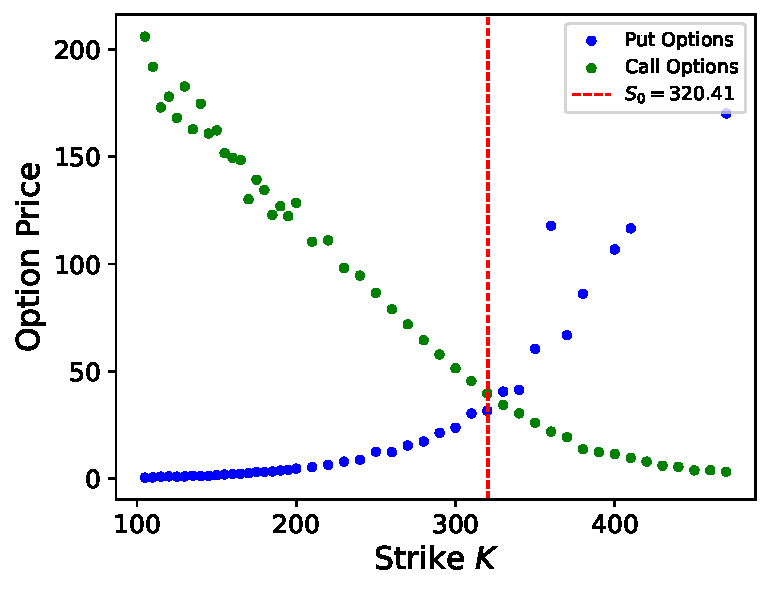
\includegraphics[width=0.5\linewidth]{option_prices.pdf}
    \caption{\textbf{Option Prices.} Market prices of the European puts and calls on \gls{jpm} with maturity January 15, 2027, quoted on November 12, 2025.}
    \label{fig:option-prices}
\end{figure}


\section{Partially Principal Protected Note}
    The \gls{pppn} balances protecting the investment against taking part in the movements of the stock.
At maturity on January 15, 2027, the investor is guaranteed to get back 90\% of the invested capital.
On top of that, the note pays a premium if \gls{jpm} ends up outside a corridor around today's price $S_0$ (see Fig.~\ref{fig:jpm-corridors}).
The premium grows with the distance from the corridor, so large moves are rewarded in either direction.

\gls{jpm} is a good fit for such a product.
Over the past year, the stock rose from \$239.56 on November 12, 2024, to \$320.41 at $t=0$, an increase of about 34\%.
Moves of this size are exactly what the premium pays for, while the investor never risks more than 10\% of the capital.

\subsection{Payoff}
The payoff of the \gls{pppn} has two parts: a protected base and a premium that depends on the stock price $S_T$ at maturity.

\paragraph{Principal Protection}
To secure 90\% of the invested amount $N$, part of the capital is invested in a zero-coupon bond.
Its present value is $0.9N e^{-rT}$, and it grows to $0.9N$ at maturity, whatever happens to the stock.

\paragraph{Premium}
Two strikes $K_1 < S_0 < K_2$ define a corridor in which no premium is paid.
Outside the corridor, the premium is proportional to how far the stock has moved:
\begin{equation}
\nonumber
    \begin{aligned}
        \text{Premium}(S_T) =
        \begin{cases}
        \frac{N}{S_0}(K_1 - S_T), & \text{if } S_T < K_1,\\[6pt]
        0, & \text{if } K_1 \leq S_T \leq K_2,\\[6pt]
        \frac{N}{S_0}(S_T - K_2), & \text{if } S_T > K_2.
        \end{cases}
    \end{aligned}
    \qquad\qquad
    \vcenter{\hbox{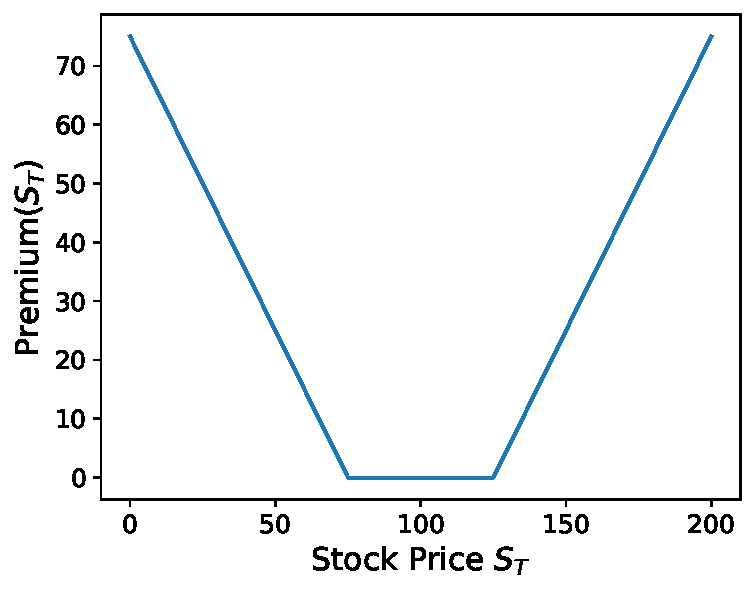
\includegraphics[width=5cm, height=4cm]{pppn_premium_payoff.pdf}}}
\end{equation}
The plot on the right shows an example with $S_0 = 100$, $K_1 = 75$ and $K_2 = 125$.
For the rest of this section, we set $N = S_0$, so that $\frac{N}{S_0} = 1$.

\subsection{Replication}
The bond provides the capital protection.
The premium is replicated by buying $\frac{N}{S_0}$ European puts with strike $K_1$ and $\frac{N}{S_0}$ European calls with strike $K_2$, both with maturity $T$.

\paragraph{Replication Cost}
The issuer also charges a margin $M$ to cover its profit and hedging costs.
We express it as a fraction $m$ of the investment, $M = mN$.
At $t = 0$, the bond, the options and the margin must add up to the amount invested:
\begin{align}
\label{eq-pppn-replication-cost}
    N = 0.9N e^{-rT} + \frac{N}{S_0}\big[EP(K_1, T) + EC(K_2, T)\big] + mN.
\end{align}

\paragraph{Choosing $K_1$ and $K_2$}
Rearranging \eqref{eq-pppn-replication-cost} gives the budget available for the two options:
\begin{align}
    EP(K_1, T) + EC(K_2, T) = S_0 \left( 1 - 0.9e^{-rT} - m \right).
    \label{eq-option-cost}
\end{align}
Strikes are only quoted in steps of 5 or 10, so this equality can usually not be met exactly.
We therefore only require the left-hand side to be at most the budget; any amount left over goes to the issuer.
Fig.~\ref{fig:valid-strike-pairs} shows all strike pairs $(K_1, K_2)$ that satisfy this condition for margins of $0.1\%$, $0.5\%$ and $1.0\%$.
Options with strikes close to $S_0$ are more expensive, because a narrow corridor makes a premium more likely.
A higher margin leaves less money for the options and therefore forces a wider corridor.

\begin{figure}
    \centering
    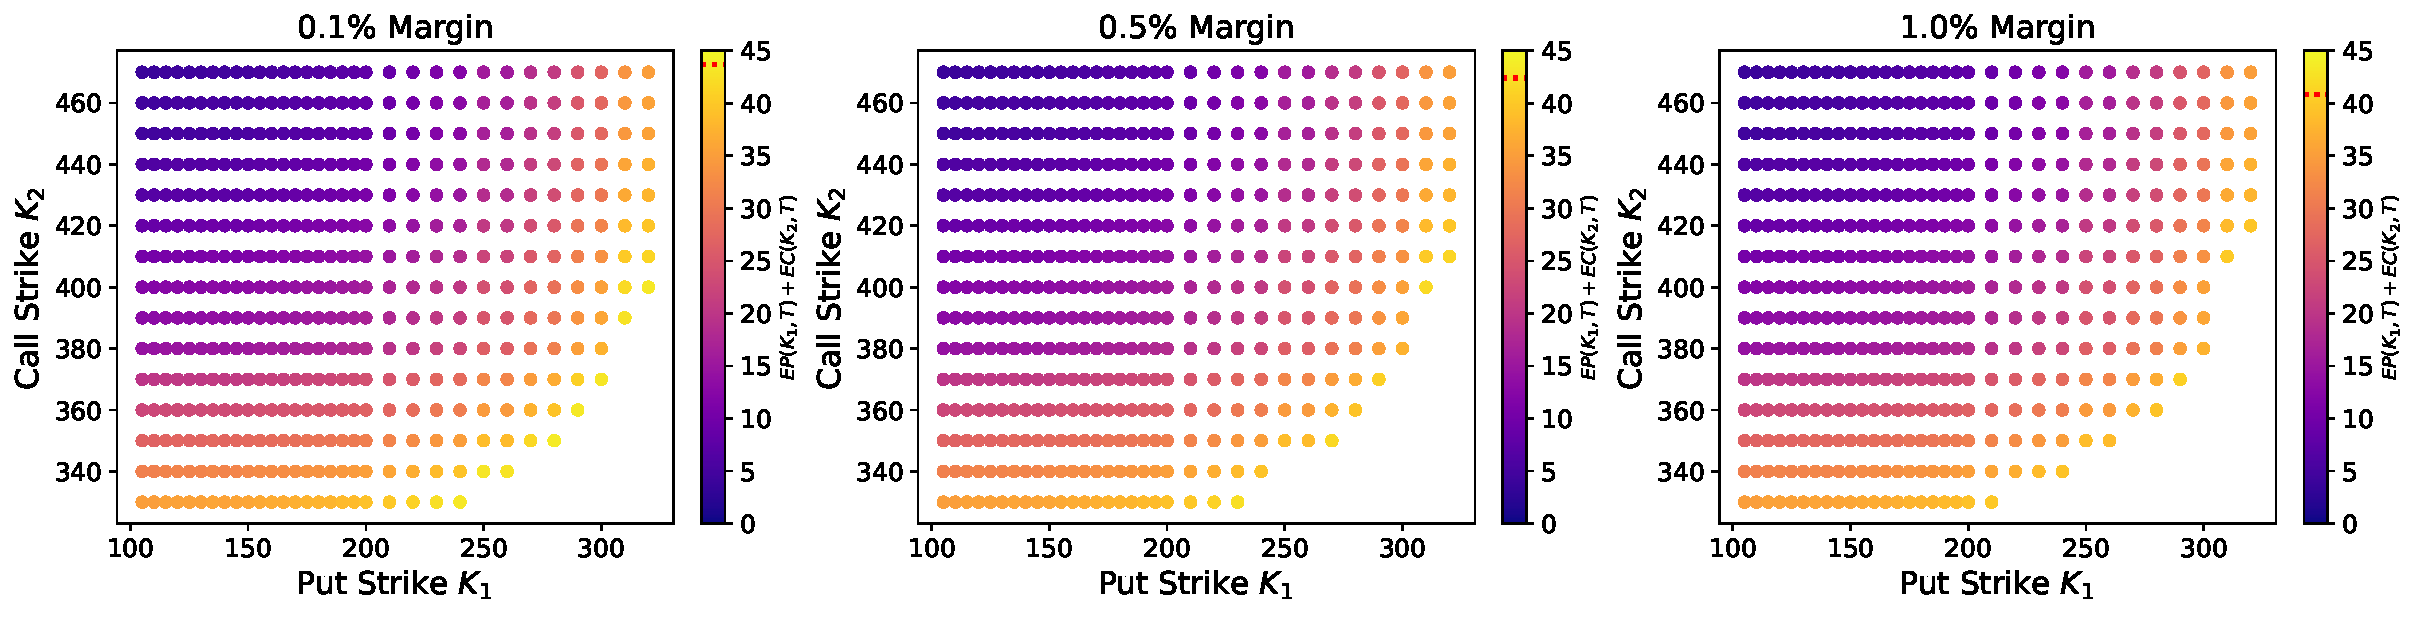
\includegraphics[width=\linewidth]{pppn_valid_strikes.pdf}
    \caption{\textbf{Valid Strike Pairs.} Strike pairs $(K_1, K_2)$ whose combined option cost fits within the budget \eqref{eq-option-cost} for margins of $0.1\%$, $0.5\%$ and $1.0\%$. The colour gives the total cost of both options, and the dotted red line in each colour bar marks the budget.}
    \label{fig:valid-strike-pairs}
\end{figure}

We choose a margin of $m = 0.5\%$, which leaves the issuer a reasonable profit while keeping the product attractive.
With $S_0 = 320.41$, $r = 3.635\%$ and $T = 1.167$, the option budget is $42.41$.
For the investor, the best strikes are those with the narrowest corridor $K_2 - K_1$.
The narrowest valid corridor has a width of 80, and among the pairs that reach it we take the one that uses most of the budget:
\begin{align}
    \nonumber
    EP(270, T) + EC(350, T) = 15.45 + 26.09 = \mathbf{41.54 \leq 42.41}.
\end{align}
The note therefore uses $K_1 = 270$ and $K_2 = 350$.
Fig.~\ref{fig:jpm-corridors} places this corridor on the price history of \gls{jpm}.

\begin{figure}[H]
    \centering
    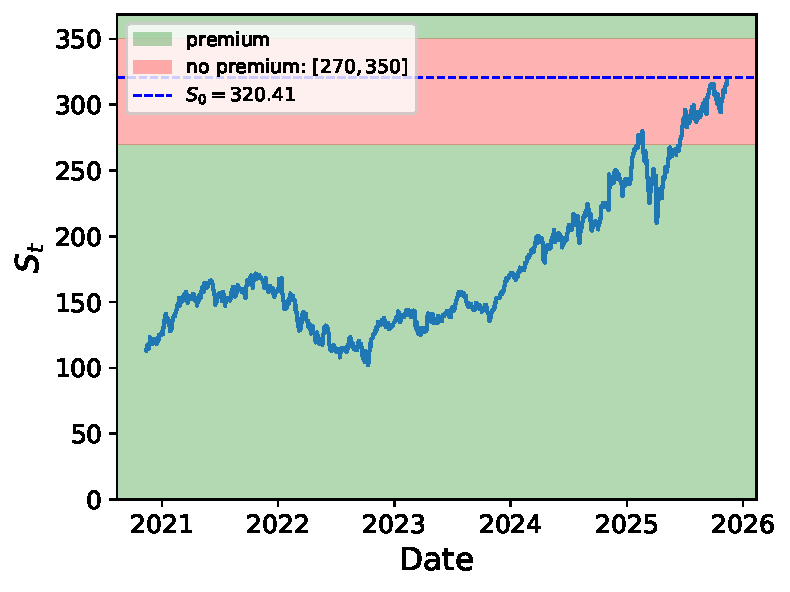
\includegraphics[width=0.5\linewidth]{pppn_jpm_corridors.pdf}
    \caption{\textbf{PPPN Corridor for JPM.} Closing prices of \gls{jpm} over the past five years together with the premium zones of the note. A premium is paid below $K_1 = 270$ and above $K_2 = 350$ (green), but not in between (red).}
    \label{fig:jpm-corridors}
\end{figure}

\subsection{Simulation}
\label{sec-pppn-simulation}
To estimate how the note might perform, we simulate \gls{jpm} as a geometric Brownian motion, discretised with the Euler--Maruyama scheme over the 294 trading days until maturity.
The drift $\mu = 23.47\%$ is the average daily log-return of \gls{jpm} over the past five years, annualised.
The volatility $\sigma = 28.9\%$ is the implied volatility of the options around the chosen strikes\footnote{\url{https://optioncharts.io/options/JPM/volatility-skew?option_type=all&expiration_dates=2027-01-15:m&strike_range=270,350}}.
The options are priced under the risk-neutral measure, but the simulation uses the real-world drift because we want to know how the product is likely to perform.
Further details are given in Appendix~\ref{appendix-monte-carlo-simulation}.

\begin{figure}[H]
    \centering
    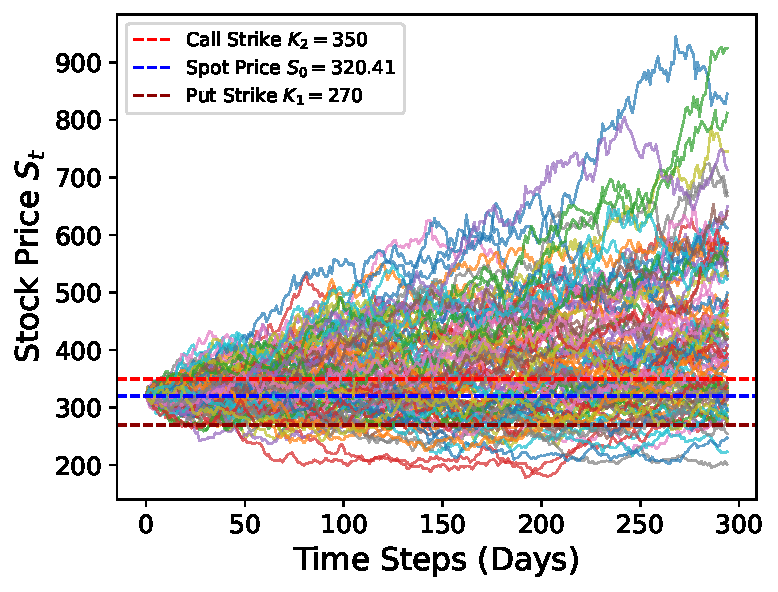
\includegraphics[width=0.5\linewidth]{pppn_simulated_paths.pdf}
    \caption{\textbf{Simulation.} 100 of the $10^4$ simulated paths of \gls{jpm} over 294 trading days. The horizontal lines mark the strikes $K_1$ and $K_2$ and the spot price $S_0$.}
    \label{fig:jpm-simulation}
\end{figure}

Fig.~\ref{fig:jpm-simulation} shows a sample of the paths.
Over $10^4$ paths, the stock leaves the corridor in $76.9\%$ of the cases, and the expected premium at maturity and its present value are
\[
    \hat{\mathbb{E}}[\text{Premium}(S_T)] = 95.57, \qquad e^{-rT}\, \hat{\mathbb{E}}[\text{Premium}(S_T)] = 91.60 > 41.54 = EP(K_1, T) + EC(K_2, T).
\]
The gap does not mean the options are cheap. It comes from the historical drift of \gls{jpm}, which is far above the risk-free rate.
The expected total payoff is
\[
    0.9N + \hat{\mathbb{E}}[\text{Premium}(S_T)] = 288.37 + 95.57 = 383.94,
\]
which corresponds to a growth factor of $\frac{383.94}{S_0} \approx 1.198$, or about $20\%$ on the initial investment.


\newpage
\section{Airbag Note}
    The Airbag Note is designed for investors who want to profit from further growth of \gls{jpm} and still be protected against moderate losses.
At maturity on January 15, 2027, the payoff depends on the final price of \gls{jpm}:
\begin{itemize}
    \item If the stock ends at or above its initial price $S_0$, the investor receives the invested capital plus a share $p$, the participation rate, of the stock's gain.
    \item If the stock ends below $S_0$ but above the airbag level $A$, the investor still receives the full capital.
    \item Only if the stock falls below the airbag level does the payoff drop, in proportion to the stock's performance.
\end{itemize}
The airbag works as a cushion against moderate declines, which makes the note suitable for risk-conscious investors who still want to take part in \gls{jpm}'s upward trend.

\subsection{Payoff}
The payoff at maturity depends on $S_T$, the participation rate $p \in (0, 1)$ and the airbag level $A \in (0, S_0)$.
It is convenient to write it as $N \cdot \varphi_{p,A}(S_T)$, where the payoff factor $\varphi_{p,A}$ scales the initial investment $N$:
\begin{equation}
\label{eq-airbag-replication-phi}
    \text{Payoff}_{p,A}(S_T) = N \cdot \varphi_{p, A}(S_T) =
    N \cdot \begin{cases}
        1 + \frac{p}{S_0} (S_T - S_0), & \text{if } S_0 \leq S_T,\\[6pt]
        1, & \text{if } A \leq S_T < S_0,\\[6pt]
        \frac{S_T}{A}, & \text{if } S_T < A.
    \end{cases}
\end{equation}
The three cases correspond to a gain ($\varphi > 1$), preserved capital ($\varphi = 1$) and a loss ($\varphi < 1$).
Working with $\varphi$ lets us analyse the product independently of the amount invested.
For this product, we set the airbag level to $A = 0.8\,S_0 = 256.33$.
The payoff is shown in Fig.~\ref{fig:airbag-payoff}.

\begin{figure}[H]
    \centering
    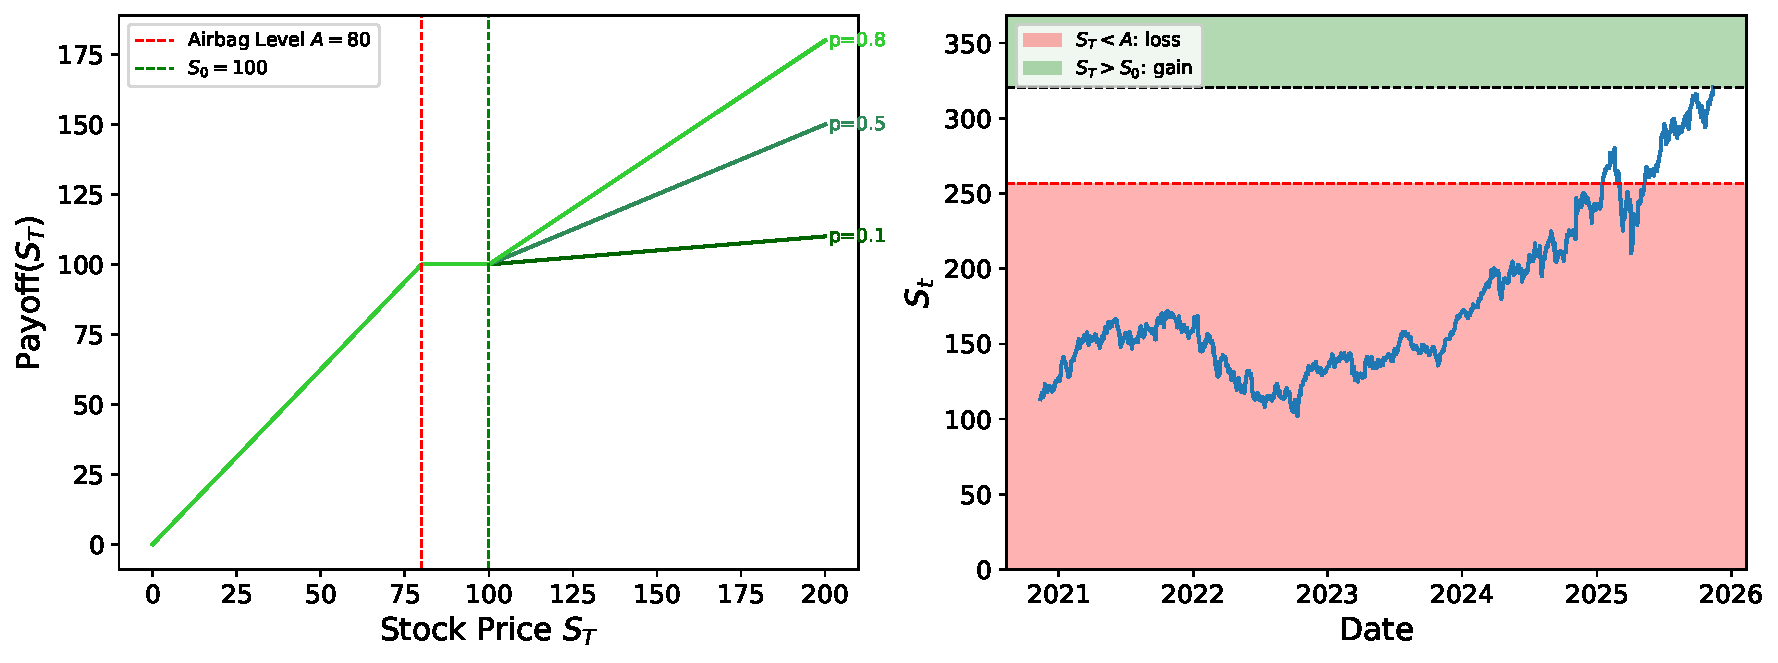
\includegraphics[width=\linewidth]{airbag_payoff.pdf}
    \caption{\textbf{Airbag Payoff.} Left: payoff for $N = 100$, $S_0 = 100$ and $A = 80$ with different participation rates. Right: closing prices of \gls{jpm} over the past five years with the airbag level $A = 256.33$ and the spot price $S_0 = 320.41$. The investor gains above $S_0$ (green), keeps the capital between $A$ and $S_0$ (white) and makes a loss below $A$ (red).}
    \label{fig:airbag-payoff}
\end{figure}

\subsection{Replication}
The payoff \eqref{eq-airbag-replication-phi} can be rewritten as
\[
    \text{Payoff}_{p, A}(S_T)
    = N \left( 1 + \frac{p}{S_0} (S_T - S_0)^+ - \frac{1}{A} (A - S_T)^+\right).
\]
This form shows the replicating portfolio directly: a zero-coupon bond that pays $N$ at maturity, a long position in $\frac{Np}{S_0}$ European calls with strike $S_0$, and a short position in $\frac{N}{A}$ European puts with strike $A$.
Including the issuer's margin $M = mN$ as before, the cost at $t = 0$ must equal the investment:
\begin{align*}
    N &= N \left( e^{-rT} + \frac{p}{S_0} EC(S_0, T) - \frac{1}{A} EP(A, T) + m \right) \\
    \Rightarrow \quad 1 &= e^{-rT} + \frac{p}{S_0} EC(S_0, T) - \frac{1}{A} EP(A, T) + m.
\end{align*}
Since both strikes are fixed, the only free parameters are the margin $m$ and the participation rate $p$.
Solving for $p$ gives a linear function of the margin:
\begin{align}
    p(m)
    = \underbrace{\left( 1 - e^{-rT} + \frac{1}{A} EP(A,T) \right) \frac{S_0}{EC(S_0,T)}}_{\alpha}
    \;+\;
    m \underbrace{\left( - \frac{S_0}{EC(S_0,T)} \right)}_{\beta}.
\end{align}
Neither $S_0 = 320.41$ nor $A = 256.33$ is a quoted strike.
We therefore interpolate the option prices linearly between the two nearest strikes: $EC(320.41, T)$ between the calls at 320 and 330, and $EP(256.33, T)$ between the puts at 250 and 260.
The resulting values are listed in Table~\ref{tab:airbag-parameters}.

\begin{figure}[t]
    \centering
    \begin{minipage}{0.48\textwidth}
        \centering
        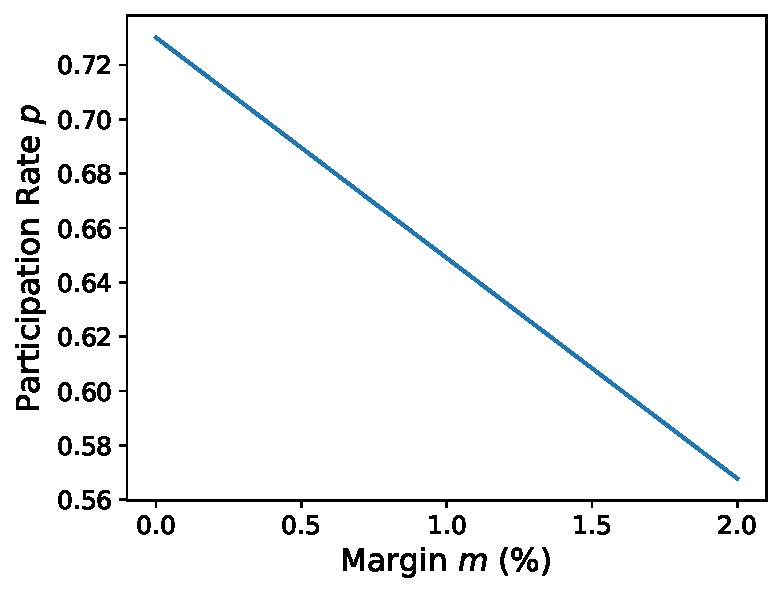
\includegraphics[width=\linewidth]{airbag_participation_vs_margin.pdf}
        \caption{\textbf{Participation vs.\ Margin.} Participation rate $p(m)$ for margins $m$ between $0\%$ and $2\%$.}
        \label{fig:airbag-participation-vs-margin}
    \end{minipage}%
    \hfill
    \begin{minipage}{0.48\textwidth}
        \centering
        \begin{tabular}{ll}
            \hline
            Parameter & Value \\
            \hline
            $r$ & 0.03635 (3.635\%) \\
            $T$ & 1.167 (14 months) \\
            $S_0$ & 320.41 \\
            $A$ & 256.33 \\
            $EC(S_0,T)$ & 39.49 \\
            $EP(A,T)$ & 12.42 \\
            \hline
            $\alpha$ & $\approx 0.730$ \\
            $\beta$ & $\approx -8.11$ \\
            \hline
        \end{tabular}
        \captionof{table}{\textbf{Parameters.} Inputs for the participation rate $p(m)$, where $\alpha$ is the intercept and $\beta$ the slope.}
        \label{tab:airbag-parameters}
    \end{minipage}
\end{figure}

Fig.~\ref{fig:airbag-participation-vs-margin} shows this linear relationship for margins between $0\%$ and $2\%$.
Without a margin, the investor would participate with $p(0) = 0.730$; at $m = 2\%$, the participation falls to $p(0.02) = 0.568$.
As for the \gls{pppn}, we choose $m = 0.5\%$, which gives a participation rate of $p(0.005) \approx 0.690$.

\subsection{Simulation}
We assess the Airbag Note with the same simulated paths as the \gls{pppn} (Sec.~\ref{sec-pppn-simulation}), this time evaluating the payoff factor $\varphi_{p,A}(S_T)$.
Over $10^4$ paths, the note ends with a gain in $76.4\%$ of the cases, preserves the capital in $16.2\%$, and makes a loss in only $7.4\%$.
The expected payoff factor is
\[
    \hat{\mathbb{E}}[\varphi_{p, A}(S_T)] = 1.234 > 1,
\]
which means an expected growth of $23.4\%$ on the initial investment.
Fig.~\ref{fig:jpm-simulation-airbag} shows 100 of the simulated paths together with the airbag level.

\begin{figure}[H]
    \centering
    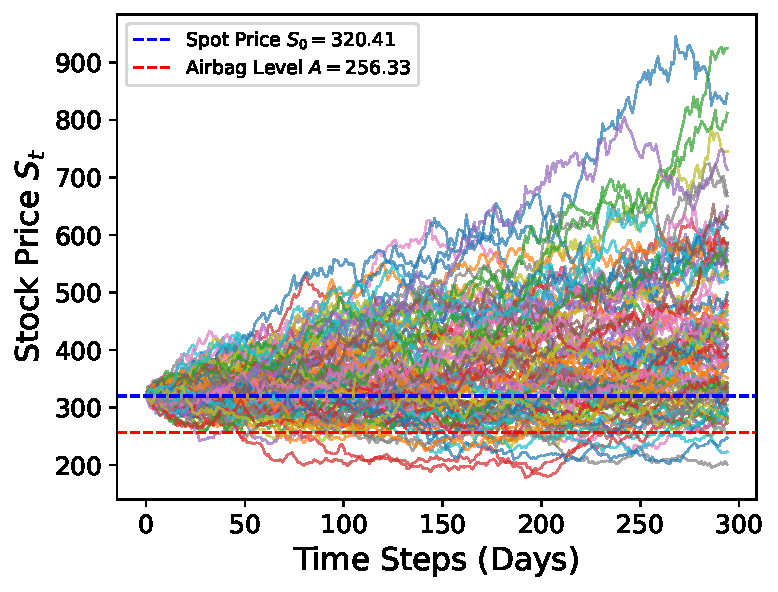
\includegraphics[width=0.5\linewidth]{airbag_simulated_paths.pdf}
    \caption{\textbf{Simulation.} 100 of the $10^4$ simulated paths of \gls{jpm}. The horizontal lines mark the airbag level $A$ and the spot price $S_0$.}
    \label{fig:jpm-simulation-airbag}
\end{figure}


\newpage
\section{Summary and Conclusion}
    In this report, we presented two structured products on \gls{jpm}, a \glsreset{pppn}\gls{pppn} and an Airbag Note, both built from a zero-coupon bond and vanilla European options.
Table~\ref{tab:structured-products-comparison} compares them.

\begin{table}[H]
    \centering
    \caption{Comparison of the two structured products.}
    \label{tab:structured-products-comparison}
    \begin{tabular}{@{}>{\raggedright\arraybackslash}p{3.5cm}>{\raggedright\arraybackslash}p{6cm}>{\raggedright\arraybackslash}p{6cm}@{}}
    \toprule
    \textbf{Aspect} & \textbf{PPPN} & \textbf{Airbag Note} \\
    \midrule
    Structure &
    90\% capital protection. Pays a premium if the stock moves out of the corridor $[270, 350]$ in either direction. &
    Full capital protection down to the airbag level $A = 256.33$. Participates partially ($p = 0.690$) in gains. \\[2mm]

    Replication &
    Zero-coupon bond worth $0.9\,N e^{-rT}$, long $EP(270,T)$ and long $EC(350,T)$. &
    Zero-coupon bond worth $N e^{-rT}$, long $EC(S_0,T)$ and short $EP(A,T)$. \\[2mm]

    Issuer margin & $0.5\%$ & $0.5\%$ \\[2mm]

    Expected growth (Monte Carlo) &
    $\hat{\mathbb{E}}[\text{Payoff}(S_T)]/N = 1.198$ &
    $\hat{\mathbb{E}}[\varphi_{p,A}(S_T)] = 1.234$ \\
    \bottomrule
    \end{tabular}
\end{table}

The \gls{pppn} combines partial capital protection with exposure to large moves in either direction.
The Airbag Note instead focuses on downside protection: the investor keeps the full capital as long as \gls{jpm} stays above the airbag level and participates in its gains, while moderate losses are absorbed.
Both products are therefore aimed at risk-conscious rather than purely risk-seeking investors, that is, at investors who want their capital protected to some degree but still want to benefit from rising prices.

Monte Carlo simulations based on the historical drift of \gls{jpm} point to favourable expected performance for both products.
For the \gls{pppn}, the present value of the expected premium is more than twice the cost of the two options.
For the Airbag Note, the expected payoff factor is above one, and a loss occurs in fewer than one in ten simulated scenarios.
These estimates rely on \gls{jpm}'s strong performance over the past five years continuing, so they should be read as indicative rather than as a forecast.


\cleardoublepage
\appendix
    \section{Monte Carlo Simulation}
\label{appendix-monte-carlo-simulation}

This appendix describes the Monte Carlo simulation used to estimate the expected payoffs of both products.
The code is available in the accompanying notebook.

\subsection{Model and Discretisation}
The stock price follows a geometric Brownian motion with drift $\mu$ and volatility $\sigma$,
\[
    dS_t = \mu S_t\, dt + \sigma S_t\, dW_t,
\]
which we discretise with the Euler--Maruyama scheme:
\[
    S_{t+\Delta t} = S_t + \mu S_t \Delta t + \sigma S_t \sqrt{\Delta t}\,\epsilon_t,
\]
where $\Delta t$ is the time step and the $\epsilon_t \sim \mathcal{N}(0,1)$ are independent.

\subsection{Procedure}
\begin{enumerate}
    \item Simulate $n$ paths of the stock price from $S_0$ up to maturity $T$.
    \item For each path $i$, evaluate the quantity of interest $X_i$ at maturity: the premium $(K_1 - S_T)^+ + (S_T - K_2)^+$ for the \gls{pppn}, and the payoff factor $\varphi_{p,A}(S_T)$ from \eqref{eq-airbag-replication-phi} for the Airbag Note.
    \item Estimate the expectation by the sample mean
    \[
        \mathbb{E}[X] \approx \hat{\mathbb{E}}[X] = \frac{1}{n} \sum_{i=1}^{n} X_{i}.
    \]
\end{enumerate}
With $n = 10^4$, the standard error is $1.12$ for the expected \gls{pppn} premium and $0.003$ for the expected Airbag payoff factor.

\subsection{Parameters}
\begin{itemize}
    \item Initial stock price: $S_0 = 320.41$
    \item Maturity: $T = 14/12 \approx 1.167$ years
    \item Number of time steps: $n_D = 294$, the NYSE trading days between November 12, 2025, and January 15, 2027
    \item Time step: $\Delta t = T / n_D$
    \item Drift: $\mu = 252 \cdot \overline{\log(S_{d+1}/S_d)} = 0.2347$, the annualised mean daily log-return of the dividend-adjusted closing price over the past five years
    \item Implied volatility: $\sigma = 0.289$
    \item Number of paths: $n = 10{,}000$
\end{itemize}

\end{document}
